\documentclass[11pt]{article}
\usepackage[margin=1in]{geometry}
\usepackage{amsmath,amssymb,amsthm,booktabs,microtype,graphicx,xcolor}
\usepackage[round,authoryear]{natbib}
\usepackage[colorlinks,linkcolor=blue!50!black,citecolor=blue!50!black]{hyperref}

\theoremstyle{definition}
\newtheorem{definition}{Definition}
\theoremstyle{plain}
\newtheorem{lemma}{Lemma}
\newtheorem{proposition}[lemma]{Proposition}
\newtheorem{conjecture}[lemma]{Conjecture}

% Every claim carries its evidence: REGISTERED (bars fixed before the data, cells
% never run before, twenty new brains), EXPLORATORY (a probe, reported to explain,
% never to support), or PROVED (within a stated model).
\newcommand{\REG}{\textnormal{\footnotesize\textsf{[REGISTERED]}}}
\newcommand{\EXP}{\textnormal{\footnotesize\textsf{[EXPLORATORY]}}}
\newcommand{\PROVED}{\textnormal{\footnotesize\textsf{[PROVED]}}}
\newcommand{\OPEN}{\textnormal{\footnotesize\textsf{[OPEN]}}}
\newcommand{\Prob}{\mathbb{P}}

\title{The Budget of a Sequence Area:\\
an Interference Load Law, a Hazard Compounded over Length,\\
and a Token Code with a Type Trace}
% AUTHOR LIST TO BE DECIDED by the authors; the library's citation order
% (CITATION.cff) is not automatically the paper's.
\author{Alif Jakir\\ \small MIT; Superintelligent Group\\ \small ORCID 0009-0000-6337-5174\thanks{Working draft. Every number
cites a registration in \texttt{research/notes/memory/PREREG\_refraction\_memory.md}
or a probe under \texttt{research/notes/memory/probes/2026-10-08/}; figures and
intervals are rebuilt from committed records by
\texttt{research/experiments/memory\_budget\_figures.py}.}}
\date{Draft, 2026-10-08}

\begin{document}
\maketitle

\begin{abstract}
A recurrent area of $n$ neurons, $k$ of them active, connected at density $p$,
with a Hebbian write and an adaptation current that recovers over $\tau$ steps,
stores sequences that it replays by itself. How much can one such area hold,
and how does it fail? On pre-registered tests at cells no run had touched, we
find: (i) one sequence of $L$ elements replays whole on every brain up to a
critical value of the interference load $\rho = Lk\ln n/(n^2p)$ --- a variable
derived to first order --- and on none a factor $1.07$--$1.15$ above it; (ii) the
recovery time must match the interval between a neuron's uses, $n/k$: matched,
it buys up to $1.65$ times the budget in small areas, and a fixed recovery time
fails large areas outright; (iii) up to $\rho = 0.09$ every sequence replays
whole however the budget is split, and past it short sequences are lost one by
one; the critical load falls linearly in the logarithm of sequence length over
three decades, as a hazard compounded over length implies, though a constant
hazard fitted on short sequences underestimates how long the longest survive;
(iv) an element that recurs across sequences is coded anew in
each, with a trace of its identity --- an intraclass correlation of about
$0.1$, fifty to a hundred times chance; (v) links between areas are budgeted by
the source area alone (exploratory). Seven predictions failed on the way and are
reported with their numbers. The results form a cost model for programs of
sequences compiled onto assembly areas.
\end{abstract}

\section{Introduction}

Neural assemblies --- sets of neurons that fire together and are formed by
Hebbian plasticity under competitive inhibition --- have been proposed as the
units of a computational calculus
\citep{papadimitriou2020brain,dabagia2025sequences}. A calculus becomes a
programming substrate only once its operations have costs: how many items an
area holds, how reliably, and how failure grows with load. For attractor
memories this is the classical capacity theory
\citep{willshaw1969nonholographic,amit1985storing,tsodyks1988enhanced}; for
sequences stored as chains of transitions it began with
\citet{sompolinsky1986temporal} and \citet{kleinfeld1986sequential}, and
adaptation as the force that moves activity along a chain goes back to latching
networks \citep{treves2005frontal}.

This paper measures the budget of one sequence area of the assembly substrate,
on a protocol in which every claim was registered before its data, at
parameter cells never run before, on twenty new random connectomes
(\emph{brains}). Its contributions:
\begin{enumerate}
\item A load law: a variable derived from interference
  (Lemma~\ref{lem:load}), a critical value predicted and confirmed at new cells,
  and its domain (Section~\ref{sec:law}).
\item The recovery time as a design parameter matched to neuron reuse, with a
  peak in small areas and a failure mode on each side (Section~\ref{sec:tau}).
\item The structure of failure: all-or-none for one long sequence, one by one
  for many short ones, unified by a hazard model whose consequences we prove
  and whose predictions we register (Section~\ref{sec:hazard}).
\item A token code: recurring elements coded apart with a measurable trace of
  their identity, and what that trace allows (Section~\ref{sec:tokens}).
\item The cost of links between areas (exploratory; Section~\ref{sec:links}),
  and a section of failed predictions (Section~\ref{sec:failed}).
\end{enumerate}

\section{The substrate and the protocol}\label{sec:methods}

\paragraph{The area.} An area has $n$ neurons, connected by a random directed
graph of density $p$ regenerated from a hash per brain. At each round the $k$
neurons with the largest input win ($k$-WTA). A synapse whose presynaptic neuron
won the previous round and whose postsynaptic neuron wins now is potentiated,
its weight multiplied by $1+\beta$ up to a clip $w_{\max} = 20$; inputs are
normalised by in-degree. The write rate is the area's convergence threshold,
$\beta = \theta = \sqrt{(1-p)\ln n/(pk)}$. A refraction bias charges every winner
by $s = \beta/2$ of its input and decays by $e^{-1/\tau}$ per round: a winner is
handicapped for about $\tau$ rounds.

\paragraph{Writing and replay.} A sequence is written one round per element:
element $e$'s stimulus fires with the recurrent input from element $e-1$'s
winners, and the write records the transition. Sequences written by separate
calls are not linked. Replay is one \emph{frozen} (no writing), \emph{masked}
(no refraction) round per step from a uniformly random half of the first
element's winners; a step succeeds if the read-out overlaps the stored state by
at least $0.3$; a sequence is \emph{whole} if every step succeeds.

\paragraph{Protocol and statistics.} Each claim below was a registration whose
bars were fixed before any run of its cells (Table~\ref{tab:methods}); smoke runs
touched only cells outside the judged set and were discarded. Reliability is
measured on a geometric ladder of loads, a fresh memory per point, and
$\rho_q$ is the load at which it falls through $q$, log-interpolated. Intervals
(Table~\ref{tab:crossings}) are percentile bootstraps over brains
\citep{efron1979bootstrap} beside the two ladder points that bracket the
crossing: where reliability jumps between adjacent ladder points on every brain
the bootstrap interval collapses, and the bracket is the honest resolution.

\section{A load law}\label{sec:law}

\begin{definition}[Independent-count model]\label{def:icm}
The $L$ stored states are independent uniform $k$-subsets; each transition adds
one count to every present synapse from one state to the next; weights
$(1+\beta)^c$ are linearised to $1+\beta c$; successors are not selected by the
connectome; normalisation is a common factor.
\end{definition}

\begin{lemma}[Interference load]\label{lem:load} \PROVED\ in the
independent-count model, to first order in $k/n$. From a state holding a
fraction $o$ of $s_t$, the members of $s_{t+1}$ receive a learned excess
$o\,\beta\sqrt{kp/(1-p)}$ standard deviations of the base input above it; every
neuron receives, from the other transitions, an excess whose variance relative
to the base input's is
\[
  \rho_\beta = \frac{Lk^2\beta^2}{n^2(1-p)},
  \qquad\text{at } \beta = \theta:\quad
  \rho = \frac{Lk\ln n}{n^2p},\ \text{signal } o\sqrt{\ln n}.
\]
\end{lemma}

\begin{proof}
The base input from $k$ active sources has variance $kp(1-p)$. A member of
$s_{t+1}$ has $okp$ active potentiated inputs worth $\beta$ each. A neuron $j$
gains $\beta$ for every other transition $s_u\to s_{u+1}$ with an active $i \in
s_u$, $j\in s_{u+1}$ and $(i,j)$ present: a Poisson number with mean $L\cdot
(k^2/n)\cdot(k/n)\cdot p$, so the excess has variance $\beta^2Lk^3p/n^2$; divide
by $kp(1-p)$.
\end{proof}

With the storage ratio $\alpha = L/n$ and coding level $f = k/n$, the law at
$\beta = \theta$ reads $\alpha_c f\ln n/p = \rho_c$, the form of the sparse
associative-memory capacity $\alpha_c f\ln(1/f) = O(1)$
\citep{willshaw1969nonholographic,tsodyks1988enhanced} with $\ln n$ in place of
$\ln(1/f)$: here the write rate, scaled with $\sqrt{\ln n}$, sets the signal.
The numerical closeness of $\rho_c$ to the Hopfield ratio $0.138$
\citep{amit1985storing} is a coincidence of normalisations.

\begin{proposition}[The load law]\label{prop:law} \REG\
In the regime $kp \ge 3\ln n$, with the mean count per synapse pair
$L(k/n)^2 = \rho kp/\ln n$ below about $0.5$, one sequence replays whole on
every brain up to a critical load and on none a factor $1.07$--$1.15$ above it
(Figure~\ref{fig:law}). Predicted at $\rho_{50} = 0.142$ from an exploratory
survey of seven cells, it was measured at $0.141$ and $0.115$ at two cells never
run (Amendment~37). Below the regime floor the cliff comes earlier ($0.089$).
\end{proposition}

\begin{figure}[t]
\centering
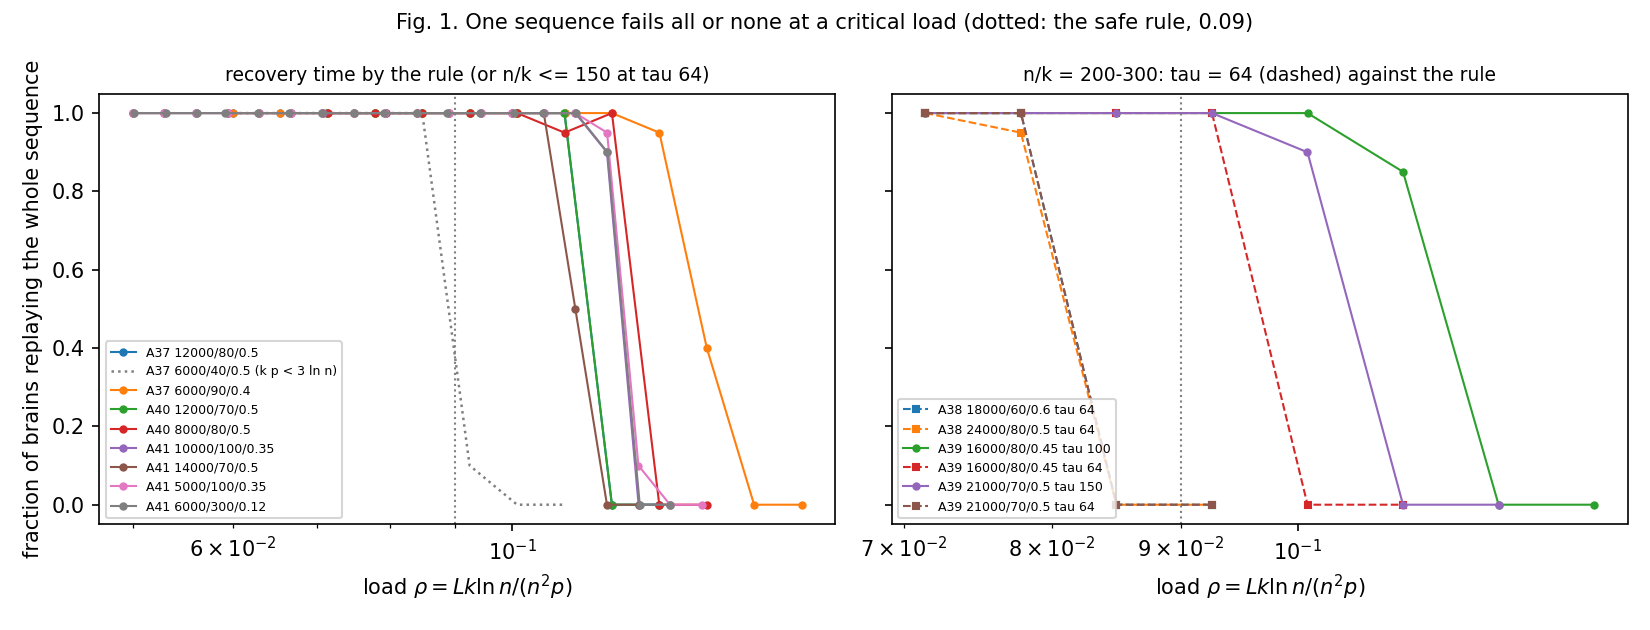
\includegraphics[width=\textwidth]{figures/fig1_load_law.png}
\caption{Reliability of one sequence against load. Left: every in-regime cell
at a recovery time matched to the area (or $n/k \le 150$ at $\tau = 64$); the
dotted grey curve is below the regime floor. Right: at $n/k = 200$--$300$ a
fixed $\tau = 64$ (dashed) puts the cliff at $0.081$--$0.097$, below the safe
rule $0.09$ (dotted line); the matched recovery time restores it. Read: the
horizontal position of each drop is the critical load; its steepness is the
all-or-none failure per brain.}
\label{fig:law}
\end{figure}

\paragraph{Where the law stops.} Two assumptions of Lemma~\ref{lem:load} fail
in measured ways. When $L(k/n)^2$ approaches one the multiplicative weights
leave the linear regime: at $kp/\ln n = 24$ replay fails at its first step from
$\rho = 0.07$ \EXP. And a reduced model of one replay step --- write-time
selection of successors, the learned transition, Poisson interference,
normalisation and $k$-WTA --- reproduces measured one-step overlap maps to
$0.02$--$0.03$ yet places the critical load at $0.23$--$0.34$ against measured
$0.12$--$0.17$ \EXP: a factor $0.48 \pm 0.05$ (mean $\pm$ sd over nine cells),
correlated $0.65$ with the measurements across cells, which removes only a
fifth of their spread. The constant is therefore measured, not derived.

\section{The recovery time is matched to reuse}\label{sec:tau}

A neuron is selected about once every $n/k$ elements. The recovery time sets
whether it is still handicapped when its next chance comes.

\begin{proposition}[A matched recovery time]\label{prop:tau} \REG
With $\tau = 64$ fixed, the critical load falls to $0.081$ at $n/k = 300$ (three
cells; Amendments~38 and 39), below the safe rule; $\tau = n/k/2$ restores it
($0.105$ and $0.114$ at $n/k = 300$ and $200$, gains $1.29$ and $1.18$ on the same
brains; Amendment~39). Against $\tau = n/k/2$, $\tau = n/k$ gives:
\begin{center}
\begin{tabular}{lcccc}
\toprule
$n/k$ & $20$ & $50$ & $100$ & $200$\\
\midrule
$\rho_{50}$, $\tau = n/k/2$ & $0.122$ & $0.123$ & $0.122$ & $0.112$\\
$\rho_{50}$, $\tau = n/k$ & $0.202$ & $0.152$ & $0.120$ & $0.102$\\
gain & $1.65$ & $1.24$ & $0.98$ & $0.91$\\
\bottomrule
\end{tabular}
\end{center}
(four cells differing in $n/k$ alone, $kp \approx 35$; Amendment~41).
\end{proposition}

\begin{figure}[t]
\centering
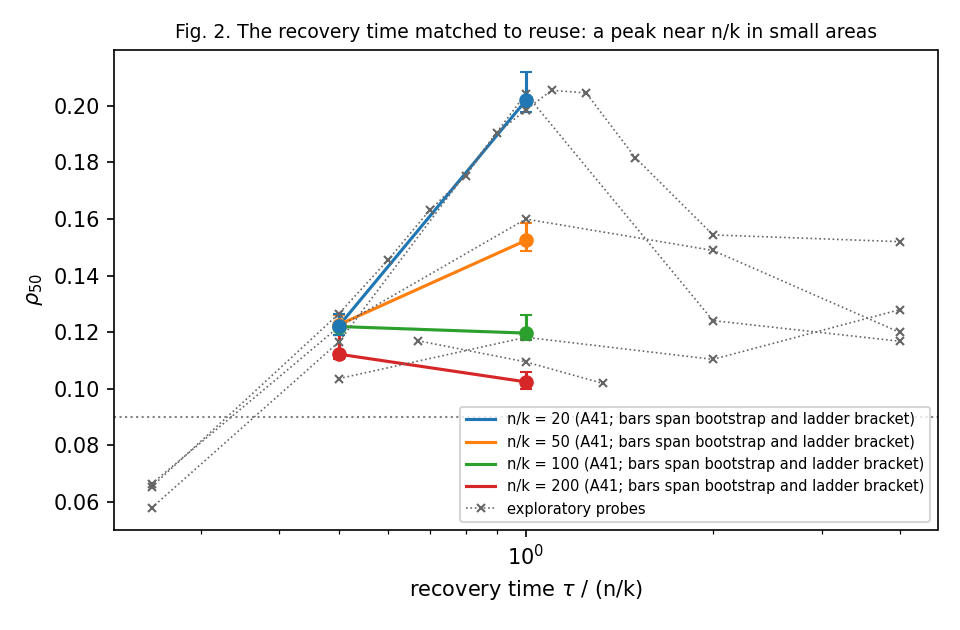
\includegraphics[width=0.72\textwidth]{figures/fig2_recovery_time.png}
\caption{Critical load against the recovery time in units of the reuse
interval $n/k$. Coloured: the registered cells of Amendment~41 (bars span the
bootstrap interval and the ladder bracket). Grey: exploratory sweeps at five
cells. Read: small areas peak near $\tau \approx n/k$; large areas are flat or
fall; below $n/k/2$ every cell collapses.}
\label{fig:tau}
\end{figure}

Both flanks of Figure~\ref{fig:tau} have a reading \EXP. Below $n/k/2$ reuse
clumps: the variance-to-mean ratio of per-neuron use counts is $7$--$12$ at
$\tau = n/k/4$, $0.3$--$0.4$ at $n/k/2$ and $0.04$--$0.08$ at $n/k$, and
$\rho_{50}$ collapses to about $0.06$ --- rich get richer. Above the optimum the
failure of a refraction that never recovers returns: where $\tau = n/k$ is the
worse choice, brains fail at step $91$--$192 \approx n/k$, the signature of the
area's neurons being used up once, rather than within a few steps of the cue as
every other failure here. Under $\tau = n/k/2$ the critical load is nearly
constant ($0.122$ from $n/k = 20$ to $100$). The design rule: $\tau = n/k$ up to
$n/k \approx 50$, $n/k/2$ from about $100$.

\section{How an area fails: a hazard compounded over length}\label{sec:hazard}

\begin{proposition}[Any split is safe; short sequences fail one by one]\label{prop:split}
\REG\ At equal total load, sequences of $16$, $64$ or thousands of elements all
replay whole up to $\rho = 0.09$ ($\rho_{90} = 0.111$--$0.132$ in every arm). Past
it one long sequence fails all or none per brain, while short ones are lost
one by one, every brain losing the same share within binomial scatter;
their $\rho_{50}$ is $1.13$--$1.20$ times the long one's (Amendment~40).
\end{proposition}

\begin{definition}[Capture and hazard]
At load $\rho$ the cue captures a sequence's first step with probability
$c(\rho)$, and every later step fails independently with probability
$h(\rho) = e^{-I(\rho)}$; then $\Prob(\text{whole}\mid\ell,\rho) =
c(\rho)\,(1-h(\rho))^{\ell-1}$. We call $I$ an escape exponent: a large-deviation
rate would require a parameter in which $I$ grows, which is not established
($kp$ is the candidate).
\end{definition}

\begin{proposition}[Consequences for one long sequence]\label{prop:ld}
\PROVED\ in the model, for $c\approx 1$, $h \ll 1$ at the cliff, and (2) $I$
linear across it. (1) $I(\rho_q(L)) = \ln L - \ln(-\ln q)$: the cliff moves
with the logarithm of what is stored. (2) $\rho_{10}-\rho_{90} \approx
3.08/|I'|$, independent of $L$ to first order.
\end{proposition}
\begin{proof}
$\Prob(\text{whole}) \approx \exp(-Le^{-I})$; set it to $q$, and difference
between $q = 0.9$ and $0.1$.
\end{proof}

Fitted after the fact to Amendment~40's record, $(c,h)$ from the $16$- and
$64$-element arms locate its long sequences' cliffs to one ladder step
(Figure~\ref{fig:hazard}). The hazard rises about three decades between
$\rho = 0.11$ and $0.13$ and then levels near $10^{-2}$ while $c$ falls: long
sequences die of the in-sequence hazard, short ones at the cue. One tension
stood: the fitted slope predicts cliffs wider ($\rho_{10}/\rho_{90} \approx
1.13$--$1.20$) than measured ($1.07$--$1.15$).

\begin{proposition}[Length costs logarithmically]\label{prop:lnl} \REG\
(the order; the slope is fitted after the run) At equal total load, $\rho_{50}$
falls strictly through sequences of $16$, $64$, $256$, $1024$ elements and one of
the whole load ($9{,}600$ and $13{,}100$ elements) at two new cells, linearly in
$\ln\ell$: by $0.0027$ and $0.0032$ per e-fold, no point more than $0.0018$ off
the line (Amendment~43, Figure~\ref{fig:hazard}).
\end{proposition}

The same amendment tested the constant-hazard model: $(c,h)$ fitted on $16$
and $64$ elements placed the $\rho_{50}$ of $256$ and $1024$ elements within $5\%$
($-1.9\%$ to $-4.7\%$) and of a whole-load sequence $4.5\%$ and $9.8\%$ low --- the
last bar failed. Point by point the miss is larger than $\rho_{50}$ shows: at
$\rho = 0.132$ the model gives $0.16$ of $256$-element sequences whole where
$0.48$ are, and none of $1024$ where $0.40$ are. Long sequences outlive a
constant hazard; failures concentrate early, plausibly in the several steps the
read-out takes to settle from a half cue. The logarithmic law of
Proposition~\ref{prop:ld} holds; its constant-hazard mechanism does not, and
the survival curve along a sequence is the measurement that separates the two.
At one cell three of the five crossings share a single ladder step, coarsened
by a rounding flaw in the registered ladder, so their order there rests on
interpolation.

\begin{conjecture}[Escape from a vanishing barrier]\label{conj:kramers} \OPEN
Replay is a Markov chain on the overlap; the cliff is the saddle-node of its
one-step map, and below it $I(\rho) \simeq A(\rho_c-\rho)^{3/2}/\sigma^2$ as for
escape over the barrier left near a saddle-node
\citep{kramers1940brownian,hanggi1990reaction} --- a continuous-time, Gaussian
result, so the exponent is a prediction here. Then
$\rho_{50}(L) \approx \rho_c - [\sigma^2(\ln L + 0.37)/A]^{2/3}$.
\end{conjecture}

\begin{figure}[t]
\centering
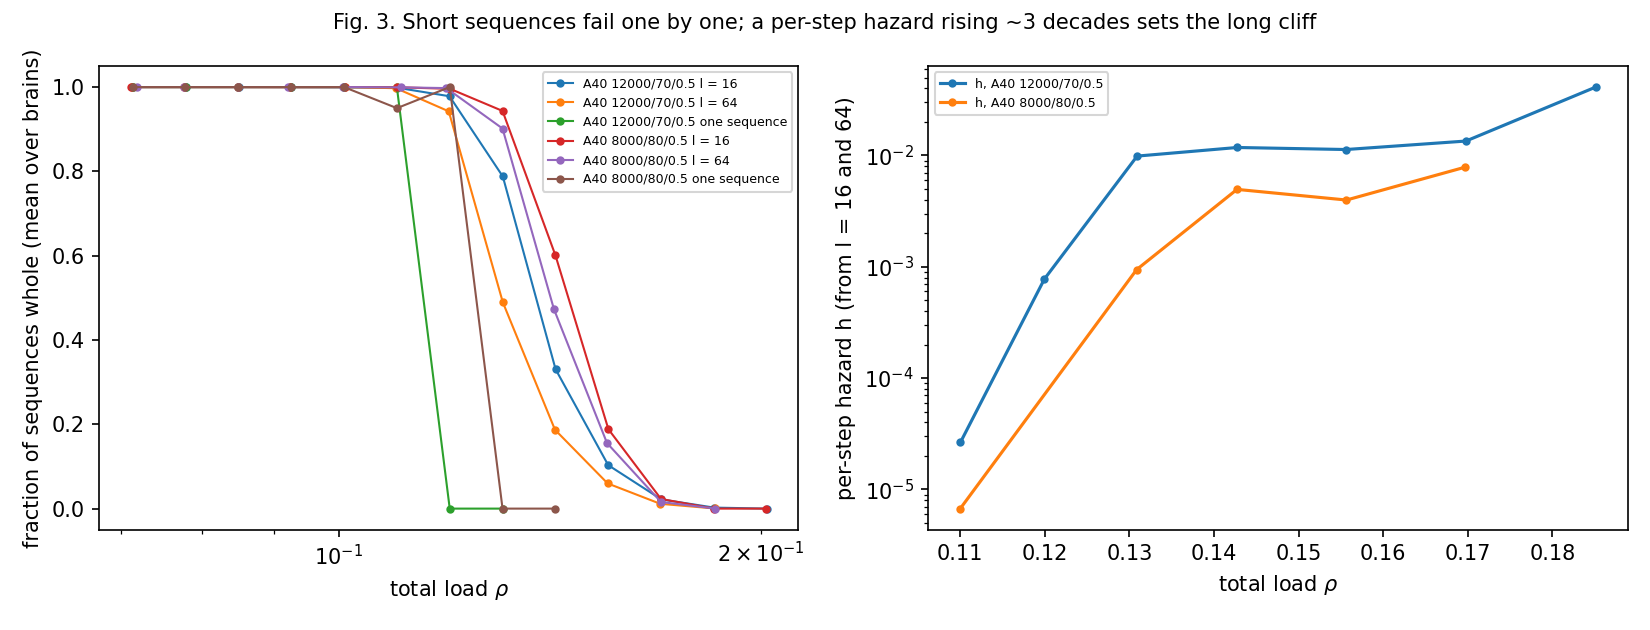
\includegraphics[width=\textwidth]{figures/fig3_hazard.png}
\caption{Left: fraction of sequences whole against total load, for one long
sequence and for many of $16$ or $64$ elements (Amendment~40; Amendment~43 when
collected). Right: the per-step hazard fitted at each load from the two short
arms. Read: the long sequence falls where the hazard crosses about $1/L$.}
\label{fig:hazard}
\end{figure}

\section{Recurring elements: a token code with a type trace}\label{sec:tokens}

\begin{proposition}[Tokens with a type trace]\label{prop:icc} \REG
Inside the safe budget, sequences whose elements recur up to five times each
cost nothing, and $5\%$ of each replay step's winners replaced at random costs
nothing; at $10\%$ noise the loss grows from $3$--$10\%$ at $\rho = 0.05$ to
$34$--$63\%$ at $0.11$. Two occurrences of an element in different sequences
share $0.072$--$0.105$ of their neurons, two different elements $0.000$--$0.002$
(Amendment~42; Figure~\ref{fig:tokens}).
\end{proposition}

Read as a variance-components model --- neuron $i$ fires in an occurrence of
element $w$ with probability $\pi_{wi}$, and the intraclass correlation (ICC) is
the share of variance in those probabilities across elements --- the code is
about $10\%$ type and $90\%$ context.

\begin{proposition}[What the trace allows]\label{prop:sb} \PROVED\ in the
variance-components model, (2) for Poisson shared counts. (1) A store summing $m$
occurrences estimates an element's type with reliability
$m\,\mathrm{ICC}/(1+(m-1)\mathrm{ICC})$ \citep{spearman1910correlation,brown1910some}:
$0.53$ at $m = 10$, $0.9$ at $m = 81$. (2) Two tokens are recognised as one
element from their shared count with $d' \approx \sqrt{\mathrm{ICC}\,k}$, about
$3$ at $k = 100$.
\end{proposition}

The first part predicts how many exposures a downstream lexical area needs; the
second, that identity becomes more legible as assemblies grow. If the shared
core is the stimulus's strongest targets, its count is sub-Poisson and $d'$
larger. Heavy recurrence (twenty uses per element) costs up to $36\%$ and fails
brain by brain, apparently by each brain's draw of sequences. We had
conjectured that a grammar --- consistent successors --- would make recurrence
cheap. An exploratory probe reversed it \EXP: with each element given $b$
allowed successors at twenty uses per element, replay produces the right
\emph{elements} (scored by the nearest stored token's identity) for $0.98$ of
sequences when successors are random, and for $0.00$--$0.39$ when $b = 1$, $2$ or
$4$; repeated transitions pull an element's tokens toward a shared code (overlap
up to $0.42$) and merge their contexts. What varies with $b$ is how often each
transition is stored, so we registered that variable against the elements'
frequency.

\begin{proposition}[Transition repetition breaks replay]\label{prop:bigram} \REG\
At a safe total load ($\rho = 0.05$), once each transition is stored about five
times, element-level replay fails on every brain at two new cells, whatever
the elements' frequency ($10$, $20$ or $40$ uses each), while random successors at
twenty uses keep $0.77$ and $0.95$ of sequences whole; repetition also raises
the overlap of an element's tokens by $0.05$--$0.06$ (Amendment~44).
\end{proposition}

\begin{proposition}[Two edges of the reuse budget]\label{prop:edges} \REG\
At two further new cells, word-level replay falls through a repetition edge
($1.00$ at one repeat per transition, $0.35$--$0.68$ at $2.8$, $\le 0.02$ at $3.7$) and a
recurrence edge (with random successors, $1.00$ at $10$--$20$ uses per element,
$\approx 0.5$ at $40$, $\le 0.09$ at $60$, failing whole brains at a time), where an
exploratory probe at a third cell had put them. The product of the two
marginal curves predicts mixed arms to a mean error of $0.05$--$0.08$; the
registered tolerance ($0.15$) was missed at one arm of ten, by $0.006$
(Amendment~45).
\end{proposition}

Two parts of the earlier registration did not resolve. Whether frequency matters at a
fixed repetition is untested: every repeated arm sits at zero, and the bar
written on their spread passes only because a spread on the floor is zero. And
frequency alone is not free: at twenty uses with random successors, whole
brains collapse ($1$ and $4$ of $20$), not those whose draws repeat bigrams most.
The implication, if the threshold proves low: one token store cannot hold a
corpus whose transitions repeat, and its statistics must be consolidated in a
separate type-level store --- the complementary-learning-systems division
\citep{mcclelland1995why}, forced here by a failure rather than assumed.

The recurrence edge can be read off the replay itself. Read each replay step's
net drive as a logit for every stored token --- the mean drive over its $k$
neurons, in units of the $k$-WTA threshold --- and call a brain's \emph{slack}
the correct next word's margin over the best other word on the steps it wins.
Brains that the standard read leaves at $0.00$ are not alike: their slack
differs, and it decides both whether they replay and how far an adaptation
during replay (each winner charged $0.1$ of its drive, decaying over $50$ steps)
recovers them.

\begin{proposition}[One margin decides replay and its rescue]\label{prop:margin} \REG\
Relative to a healthy brain's at the same cell (reuse $U = 10$), slack $x$ places
every brain on one logistic: replay holds above $x \approx 0.75$--$0.76$ at four
cells, two of them new ($0.748$, $0.760$ against the probes' $0.760$,
$0.765$), and read-time adaptation lowers the requirement to $0.64$--$0.65$.
Collapsed brains are rescued in the order of their slack (Spearman $0.86$,
$0.87$ over $51$ and $69$ brain-arms), and the size of their rescue, predicted
from slack before it was applied, was within $0.03$ and $0.05$ of the observed
(Amendment~48). The attractor's own stability predicts nothing (exploratory):
the collapse is a loss of signal margin, not a deep false well.
\end{proposition}

Where the margin goes is visible in the store itself. Compared pairwise with no
replay at all, collapsed brains hold tokens of \emph{different} words written
onto one assembly, healthy brains none; in write order the captures begin at a
brain-specific point and then accelerate, and once they do, sequences written
cleanly before them fail too (exploratory). Writing is itself a recurrent step,
so a captured assembly pulls later writes in. That suggests a control at the
source --- the function the dentate gyrus is held to serve before CA3 stores a
pattern \citep{mcclelland1995why}.

\begin{proposition}[Separation at write prevents the collapse]\label{prop:separation} \REG\
Preview each write, and inhibit for that write the neurons of any stored token
it would overlap by $0.3$ or more, using no word identity. At two new cells,
$50$ uses per element go from $0.17$ and $0.07$ to $0.99$, and $60$ uses from
$0.00$ to $0.91$; no brain is left collapsed, a healthy store is untouched, and
under $2\%$ of writes are intervened on (Amendment~49). The recurrence edge of
Proposition~\ref{prop:edges} belongs to the write policy, not the substrate.
The check compares each write with every stored token; a circuit that
computes it is not yet tested.
\end{proposition}

Part of that lift was not capture: the check also separated each sequence's
first element, which the stimulus alone writes, nearly identically for
sequences that share a first word, so it disambiguated cues; on later writes
only, the same oracle reaches $0.65$ (exploratory). A circuit that needs no
oracle does better. Before each write, compare what memory predicts --- a
projection by recurrence alone --- with the write itself, as CA1 is held to
compare CA3's recall with cortical input \citep{vinogradova2001hippocampus,lisman2005hippocampal};
if they agree on half their winners, inhibit the predicted cells for that write.

\begin{proposition}[A local comparator separates at write]\label{prop:comparator} \REG\
At two new cells, the comparator lifts $50$ uses per element from $0.10$ to
$0.94$--$0.96$ and $60$ from $0.00$--$0.01$ to $0.87$--$0.90$, leaves no brain
collapsed and a healthy store untouched, acts on $2$--$3\%$ of writes and
catches $78$--$84\%$ of the oracle's captures (Amendment~50). Suppressing
recurrence globally during writing instead --- a cholinergic encoding mode
\citep{hasselmo2006role} --- destroyed even a healthy store in the
exploratory probes: recurrence at write is what makes the token code.
\end{proposition}

\begin{figure}[t]
\centering
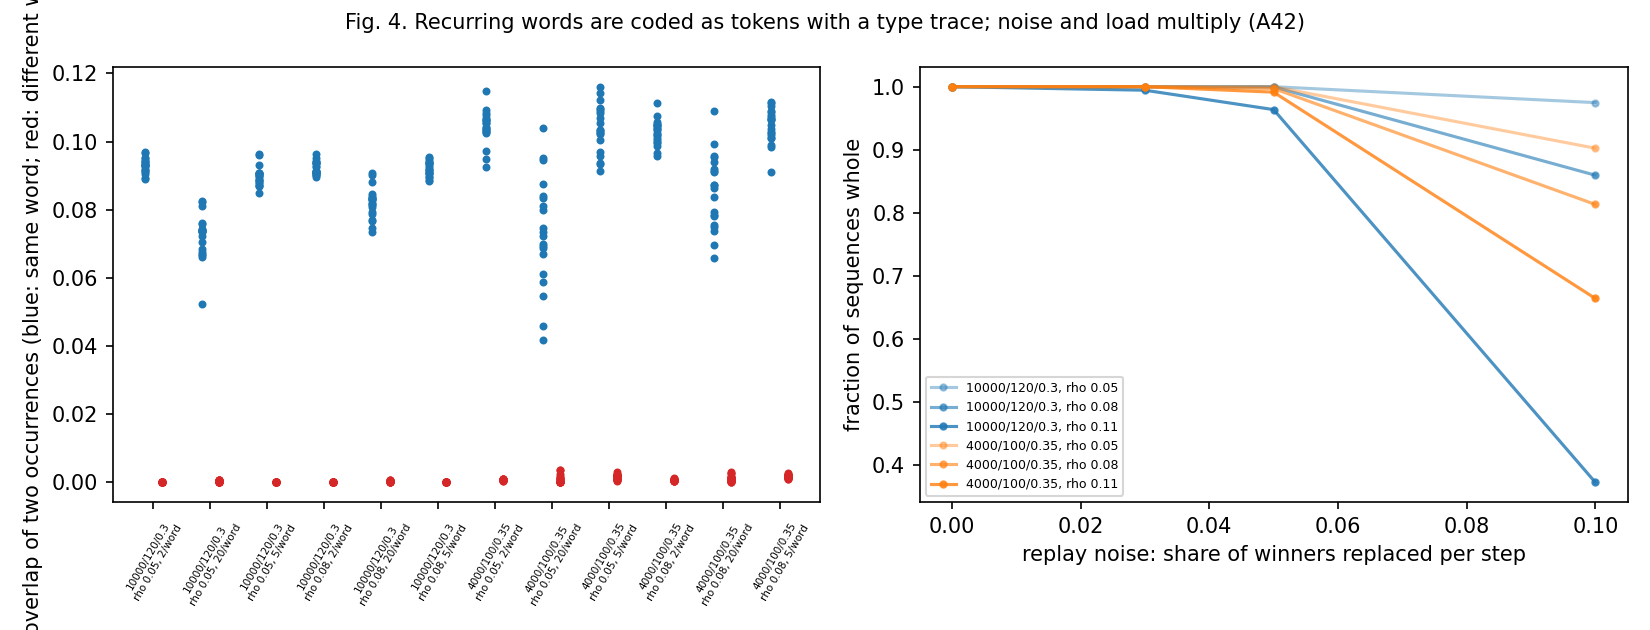
\includegraphics[width=\textwidth]{figures/fig4_tokens_noise.png}
\caption{Left: per-brain overlap of two occurrences of the same element (blue)
and of two different elements (red), by load and uses per element. Right:
fraction of sequences whole against replay noise at three loads. Read: same
occurrences share about a tenth of their neurons, different ones almost none;
noise costs nothing at $5\%$ inside the budget and multiplies with load at
$10\%$.}
\label{fig:tokens}
\end{figure}

\section{Links between areas}\label{sec:links}

A hierarchy of areas --- a chunk area whose states point at chunks stored once
in a sequence area --- replays sequences of sequences (Amendment~33), and
its first point of failure is the fiber of links from chunk-area states to
chunk starts. In an exploratory sweep \EXP\ ($k = 60$, $p = 1/2$, ten brains,
two sizes of each area), the associations at which half the starts are evoked
are $1810$ and $2400$ (for $16$ and $64$ targets) at $n_C = 2000$ and $2455$ and
about $4000$--$4100$ at $n_C = 4000$, whatever the sequence area's size: doubling
$n_S$ changes them by under $2\%$ (Figure~\ref{fig:links}). Failure is gradual,
and the wrong target that wins is the one with the most links. We conjecture
that a link budget is a law of the source area alone \OPEN, which would bound a
hierarchy's depth by its chunk areas.

\begin{figure}[t]
\centering
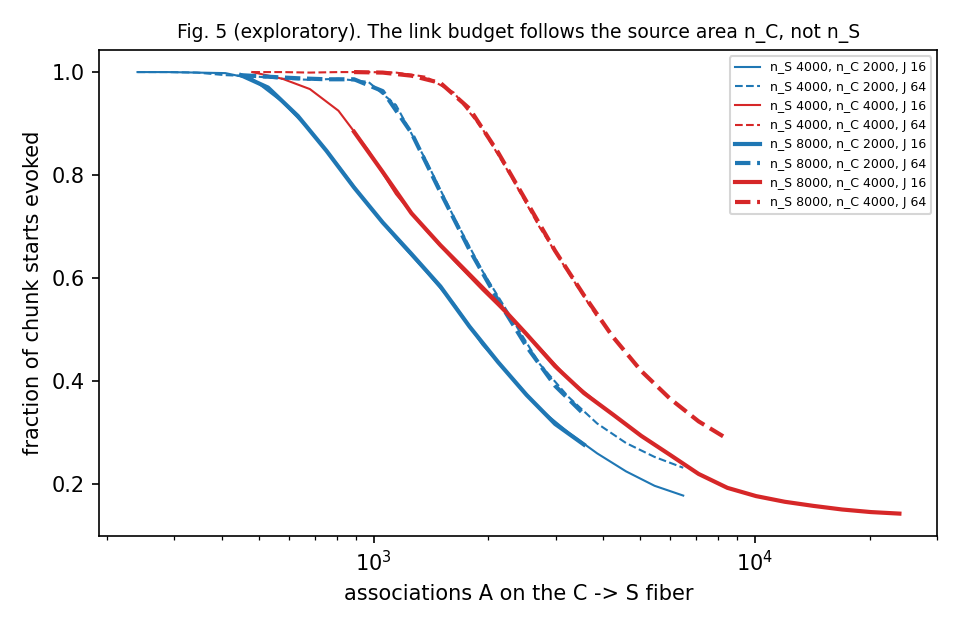
\includegraphics[width=0.72\textwidth]{figures/fig5_links.png}
\caption{Fraction of chunk starts evoked against associations stored on the
link fiber (exploratory). Colour: source-area size $n_C$; line width:
target-area size $n_S$; dashes: $64$ targets. Read: curves of equal colour
coincide; the target area's size does not matter.}
\label{fig:links}
\end{figure}

\section{What failed}\label{sec:failed}

Seven predictions or hypotheses failed and redirected the work. (1) The
constant: registered to hold at $n/k = 300$, it fell to $0.081$ with a fixed
recovery time, and the safe rule broke (Amendment~38, three of four bars
failed); the failure located the recovery time. (2) A rescaling of $\rho$ with
$\ln(n/k)$ halved the residuals of the cells already measured and failed at new
cells with small $n/k$ (predicted $0.20$--$0.23$, measured $0.10$--$0.12$) \EXP.
(3) The hypothesis that every parameter acts through the dispersion $\kappa$ of
interference --- $\rho_{50}\kappa$ constant --- was measured before it was
registered and fails: $\rho_{50}\kappa$ ranges $0.12$--$0.56$; dispersion explains
the collapse at short $\tau$ ($\kappa = 8.5$) but not the peak, where $\kappa$
moves from $1.31$ to $0.95$ while $\rho_{50}$ rises $1.66$-fold \EXP. (4) A first
draft of Amendment~40 asked for equal $\rho_{50}$ across splits; an exploratory
probe showed graded failure, and the bars were rewritten before the judged run.
(5) A constant per-step hazard, fitted on short sequences, was registered to
place a whole-load sequence's cliff within $5\%$ and placed it $9.8\%$ low at one
cell (Amendment~43): the hazard is not constant along a sequence.
(6) The product law of the reuse budget was registered to predict every mixed
arm within $0.15$ and missed one of ten by $0.006$ (Amendment~45).
(7) A control for the recurrence collapse --- adaptation during replay, which
every other replay here lacks --- was registered to raise a cell's mean by $0.15$,
to leave the repetition failure untouched and to turn harmful when strong; it
passed only its no-harm bar (Amendment~46). The cell mean depends on how many
brains collapse, and the size missed at one cell ($+0.14$); paired by brain after
the run, every brain that changed improved ($36$ of $36$, none worse), collapsed
brains rising from $0.01$ to $0.39$ --- a real effect whose size, specificity and
window the registration did not establish.
Registered again paired and conditional on collapse (Amendment~47), every
failing brain was helped and none harmed ($52$ of $54$ gained, none lost), a
healthy memory untouched and the repetition failure barely moved; the lift
of collapsed brains ($0.18$--$0.23$) again missed its registered size at one cell.
The size was then predicted, not guessed: a logit-lens margin measured before
adaptation placed it within $0.05$ at two new cells (Amendment~48,
Proposition~\ref{prop:margin}).

\section{Discussion: a cost model}\label{sec:discussion}

\begin{center}
\begin{tabular}{p{0.58\textwidth}p{0.32\textwidth}}
\toprule
Rule & Evidence \\
\midrule
Load variable $\rho = Lk\ln n/(n^2p)$; $\rho_\beta$ in general & proved in a model (Lemma~\ref{lem:load}) \\
Recovery time $n/k$ to $n/k \approx 50$, $n/k/2$ from $\approx 100$ & registered (Prop.~\ref{prop:tau}) \\
Total load $\le 0.09$: every sequence whole, any split & registered (Props.~\ref{prop:law}, \ref{prop:split}) \\
$\le 5$ uses per element and $\le 5\%$ noise cost nothing there & registered (Prop.~\ref{prop:icc}) \\
Critical load falls $\approx 0.003$ per e-fold of sequence length & registered order, fitted slope (Prop.~\ref{prop:lnl}) \\
Past it: losses per sequence; constant hazard good to $1024$ elements, pessimistic beyond & registered (one bar failed) \\
Element identity: Spearman--Brown, $d' \approx \sqrt{\mathrm{ICC}\,k}$ & proved in a model; ICC registered \\
Reuse: edges near $2.8$ repeats per transition and $40$ uses per element; product law approximate & registered (Props.~\ref{prop:bigram}, \ref{prop:edges}) \\
Read-time adaptation helps every failing brain, harms none & registered \\
Replay holds above a relative logit margin $\approx 0.76$; adaptation lowers it to $\approx 0.65$ and its rescue is predicted & registered (Prop.~\ref{prop:margin}) \\
Separation at write ($<2\%$ of writes) removes the recurrence edge: $60$ uses per element replay at $0.91$ & registered (Prop.~\ref{prop:separation}) \\
A local comparator (recall vs write) does it without an oracle, on $2$--$3\%$ of writes & registered (Prop.~\ref{prop:comparator}) \\
Links: source-area law & exploratory \\
\bottomrule
\end{tabular}
\end{center}

A compiler that allocates sequences to areas can now ask, before running a
program, whether an area will replay it, and with what loss past its budget.
The failures of long sequences and the cheapness of short ones favour
chunking \citep{miller1956magical}; the token code places identity in a second
area; and the link budget makes the chunk area, not the sequence area, the
bottleneck of depth. Three things limit the reach of these results: the
critical value is measured, not derived (the reduced model is a factor two off);
the substrate is an abstraction (hash-regenerated random graphs, $k$-WTA in
place of inhibitory dynamics), whose universality class is untested; and no
program at language scale has yet been compiled and run inside its predicted
budget.

\appendix
\section{Registrations and intervals}

\begin{table}[h]
\centering\small
\begin{tabular}{p{0.2\textwidth}lp{0.38\textwidth}p{0.2\textwidth}}
\toprule
Claim & Amendment & Judged cells $(n,k,p)$ & Bars \\
\midrule
Load law & 37 & $(6000,90,0.4)$, $(12000,80,0.5)$ & R1--R3 pass \\
Constant at $n/k = 300$ & 38 & $(18000,60,0.6)$, $(24000,80,0.5)$ & K1, D1, S1 fail; S2 pass \\
Matched recovery time & 39 & $(21000,70,0.5)$, $(16000,80,0.45)$ & T1--T4 pass \\
Any split & 40 & $(8000,80,0.5)$, $(12000,70,0.5)$ & A1--A3 pass \\
The recovery-time peak & 41 & $(6000,300,0.12)$, $(5000,100,0.35)$, $(10000,100,0.35)$, $(14000,70,0.5)$ & P1--P4 pass \\
Recurrence and noise & 42 & $(4000,100,0.35)$, $(10000,120,0.3)$ & W1, W2, N1, N2 pass \\
Hazard predictions; length & 43 & $(10000,70,0.5)$, $(8000,50,0.7)$ & K1, K2, K4 pass; K3 fail \\
Transition repetition & 44 & $(9000,110,0.33)$, $(12000,80,0.45)$ & G1, G4 pass; G3 vacuous; G2 fail \\
Two edges of reuse & 45 & $(10000,75,0.48)$, $(7000,60,0.6)$ & S1 pass; S2 fail (by $0.006$) \\
Read-time adaptation & 46 & $(11000,80,0.45)$, $(8000,60,0.6)$ & H2 pass; H1, H3, H4 fail \\
Read-time rescue, paired & 47 & $(9000,70,0.5)$, $(13000,90,0.4)$ & Q1, Q3 pass; Q2, Q4 fail \\
One logit margin & 48 & $(7500,55,0.6)$, $(12500,85,0.42)$ & M1--M4 pass \\
Separation at write & 49 & $(9500,70,0.5)$, $(11500,80,0.45)$ & W1--W6 pass \\
Local comparator & 50 & $(8500,65,0.5)$, $(12000,85,0.43)$ & C1--C6 pass \\
\bottomrule
\end{tabular}
\caption{The registrations behind each claim; seeds 522--801, twenty new brains
per amendment.}
\label{tab:methods}
\end{table}

\begin{table}[h]
\centering\scriptsize
\begin{tabular}{llllll}
\toprule
Amendment & Cell $(n,k,p)$ & Arm & $\rho_{90}$ & $\rho_{50}$ [bootstrap] \{ladder bracket\} & $\rho_{10}$ \\
\midrule
A37 & (12000, 80, 0.5) & tau 64 & 0.111 & 0.115 [0.115, 0.115] \{0.110, 0.120\} & 0.119 \\
A37 & (6000, 40, 0.5) & tau 64 & 0.086 & 0.089 [0.089, 0.090] \{0.085, 0.093\} & 0.093 \\
A37 & (6000, 90, 0.4) & tau 64 & 0.132 & 0.140 [0.138, 0.145] \{0.131, 0.143\} & 0.152 \\
A38 & (18000, 60, 0.6) & tau 64 & 0.078 & 0.081 [0.081, 0.081] \{0.078, 0.085\} & 0.084 \\
A38 & (24000, 80, 0.5) & tau 64 & 0.078 & 0.081 [0.081, 0.081] \{0.078, 0.085\} & 0.084 \\
A39 & (16000, 80, 0.45) & tau 100 & 0.107 & 0.114 [0.113, 0.115] \{0.110, 0.120\} & 0.119 \\
A39 & (16000, 80, 0.45) & tau 64 & 0.093 & 0.097 [0.097, 0.097] \{0.093, 0.101\} & 0.100 \\
A39 & (21000, 70, 0.5) & tau 150 & 0.101 & 0.105 [0.104, 0.105] \{0.101, 0.110\} & 0.109 \\
A39 & (21000, 70, 0.5) & tau 64 & 0.078 & 0.081 [0.081, 0.081] \{0.078, 0.085\} & 0.084 \\
A40 & (12000, 70, 0.5) & l = 16 & 0.124 & 0.138 [0.138, 0.138] \{0.131, 0.143\} & 0.156 \\
A40 & (12000, 70, 0.5) & l = 64 & 0.121 & 0.131 [0.130, 0.131] \{0.120, 0.131\} & 0.151 \\
A40 & (12000, 70, 0.5) & one sequence & 0.111 & 0.115 [0.115, 0.115] \{0.110, 0.120\} & 0.119 \\
A40 & (8000, 80, 0.5) & l = 16 & 0.132 & 0.146 [0.146, 0.146] \{0.143, 0.156\} & 0.163 \\
A40 & (8000, 80, 0.5) & l = 64 & 0.131 & 0.142 [0.141, 0.142] \{0.131, 0.142\} & 0.161 \\
A40 & (8000, 80, 0.5) & one sequence & 0.121 & 0.125 [0.125, 0.125] \{0.120, 0.131\} & 0.130 \\
A41 & (10000, 100, 0.35) & tau 100 (1.0 n/k) & 0.113 & 0.120 [0.117, 0.122] \{0.119, 0.126\} & 0.126 \\
A41 & (10000, 100, 0.35) & tau 50 (0.5 n/k) & 0.119 & 0.122 [0.121, 0.122] \{0.119, 0.126\} & 0.125 \\
A41 & (14000, 70, 0.5) & tau 100 (0.5 n/k) & 0.107 & 0.112 [0.110, 0.114] \{0.112, 0.119\} & 0.118 \\
A41 & (14000, 70, 0.5) & tau 200 (1.0 n/k) & 0.093 & 0.102 [0.101, 0.104] \{0.100, 0.106\} & 0.108 \\
A41 & (5000, 100, 0.35) & tau 25 (0.5 n/k) & 0.119 & 0.123 [0.122, 0.123] \{0.119, 0.126\} & 0.126 \\
A41 & (5000, 100, 0.35) & tau 50 (1.0 n/k) & 0.141 & 0.152 [0.149, 0.154] \{0.150, 0.159\} & 0.162 \\
A41 & (6000, 300, 0.12) & tau 10 (0.5 n/k) & 0.119 & 0.122 [0.121, 0.123] \{0.119, 0.126\} & 0.125 \\
A41 & (6000, 300, 0.12) & tau 20 (1.0 n/k) & 0.191 & 0.202 [0.198, 0.204] \{0.200, 0.212\} & 0.210 \\
\bottomrule
\end{tabular}

\caption{Every registered crossing with its bootstrap interval over brains and
the ladder points that bracket it.}
\label{tab:crossings}
\end{table}

\bibliographystyle{plainnat}
\bibliography{../../_shared_assets/bibliography/references}

\end{document}
